%==============================================================================
% File: 	analysis.Rnw 
% Author: Peter DeWitt, peter.dewitt@ucdenver.edu 
% Date:   Nov 2013
% 
% Purpose:	analysis of the external beam radiation project : example project
% for showing the use of R, LaTeX, and knitr
%
% Change log:
% 13 Nov 2013 - file created
% 
%==============================================================================




\section{Analysis and Results \label{sec:analysis}}

\subsection{Data Set Description}
%{{{

The data contained information on the following variables and
the levels for each.  There is additional information in the data set on the
Gleason scores.  For patients with a Gleason score of 7, the primary-secondary
values of `3+4' and `4+3' are available.  The following analysis uses a Gleason Score
variable with the total score used in all cases save GS 7 which is reported with
primary-secondary delineations.  Table~\ref{tab:data_summary} on
page~\pageref{tab:data_summary} report the observed data set overall and by
Gleason score.  There is a total of 
19,039
data records avaiable for analysis.





%}}}

\subsection{Seven Year Survival}
%{{{

Table~\ref{tab:gleason_km_surv_est} reports the Kaplan-Meier estimates for
survival at 88 months, the maximum follow up time observed, for each Gleason score.  
The estimated survival by primary-secondary patterns for 
Gleason scores 7 is also reported.  







%}}}

\subsection{Primary-Secondary Levels or Sums?}
%{{{
In this section of the analysis we investigate if there is any difference in the
OS or PCSS between the primary-secondary levels by Gleason score.
Results of six separate Cox PH regression models, one to compare the
relative difference in the hazard for OS and PCSS between the two levels of
delineation in each Gleason 7, 8, or 9 score,  are reported in
Table~\ref{tab:Gleason_primary_secondary_univar}.    These results indicate
there is no statistically significant differences in the hazards between the
different delineations for Gleason 8 and 9 for either OS or PCSS.  There is a
statistically significant difference in the hazard between GS 7 (4+3) and GS 7
(3+4).

Figure~\ref{fig:OS_PCSS_GS} are the Kaplan-Meier survival curves for overall and
prostate cancer survival for each Gleason score.
Figure~\ref{fig:primary_secondary_km} show the Kaplan-Meier plots for the
primary/secondary patterns within Gleason 7, 8, and 9.  Table~\ref{tab:n_evnets}
report the number of patients at risk overall and the number of deaths observed
for each Gleason score.




\begin{figure}
  \begin{subfigure}[t]{0.48\textwidth} 
\begin{knitrout}
\definecolor{shadecolor}{rgb}{0.969, 0.969, 0.969}\color{fgcolor}

{\centering 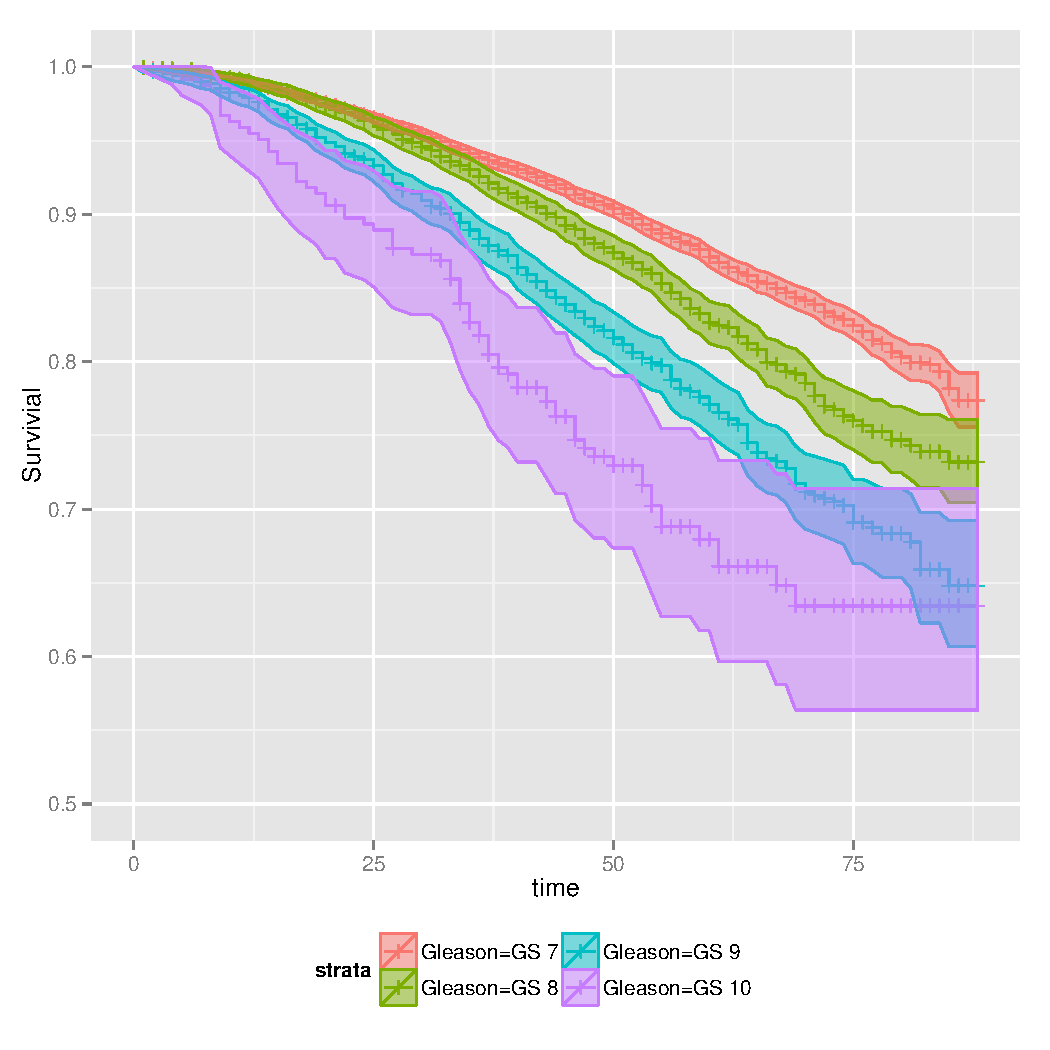
\includegraphics[width=\maxwidth]{figure/OS_GS} 

}



\end{knitrout}

    \caption{(OS\_GS.pdf) KM plot for OS by Gleason Score.}
    \label{fig:OS_GS}
  \end{subfigure}
  ~
  \begin{subfigure}[t]{0.48\textwidth} 
\begin{knitrout}
\definecolor{shadecolor}{rgb}{0.969, 0.969, 0.969}\color{fgcolor}

{\centering 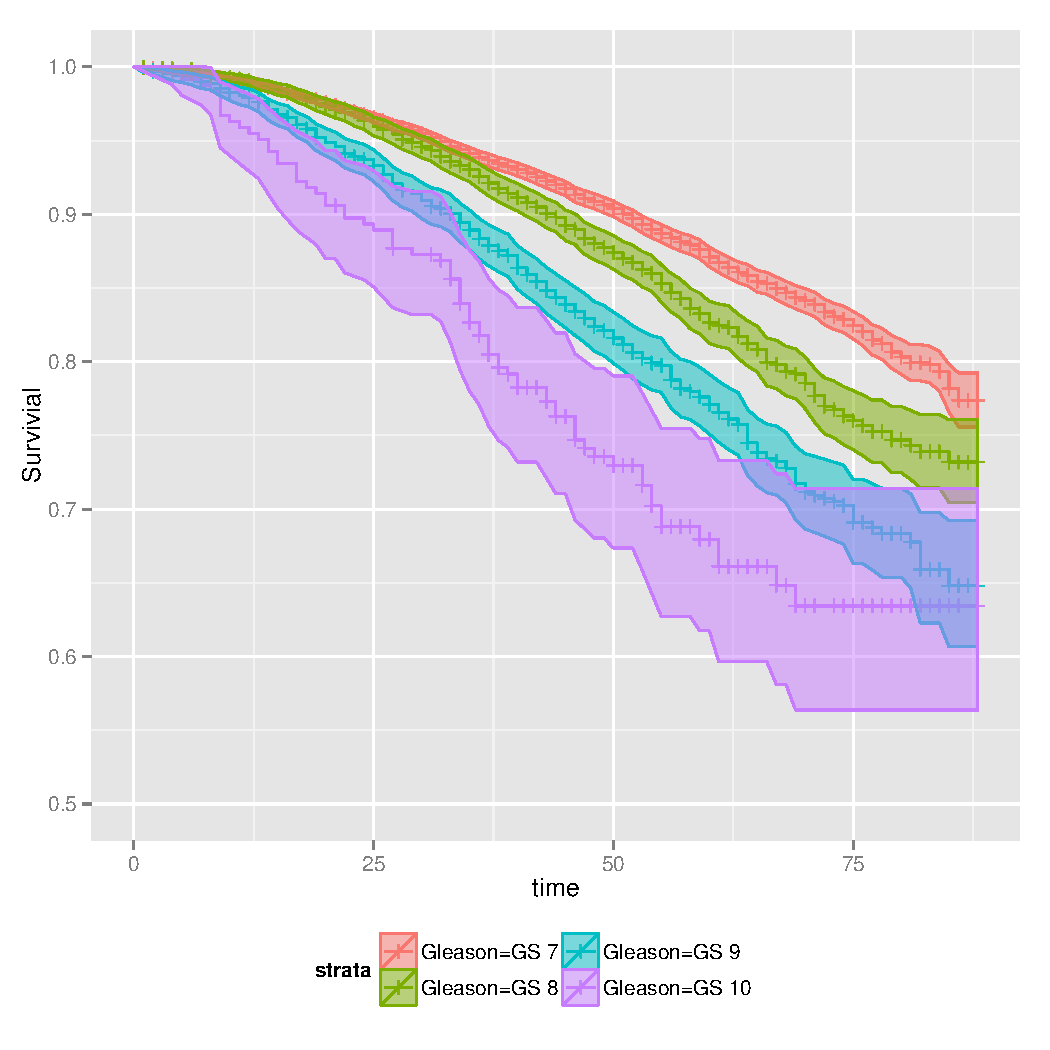
\includegraphics[width=\maxwidth]{figure/PCSS_GS} 

}



\end{knitrout}

    \caption{(PCSS\_GS.pdf) KM plot for PCSS by Gleason Score.}
    \label{fig:PCSS_GS}
  \end{subfigure}
  \caption{KM plots for OS and PCSS by Gleason Score.}
  \label{fig:OS_PCSS_GS}
\end{figure}

% KM plots
%{{{




\begin{figure}
  \begin{subfigure}[t]{0.48\textwidth}
\begin{knitrout}
\definecolor{shadecolor}{rgb}{0.969, 0.969, 0.969}\color{fgcolor}

{\centering 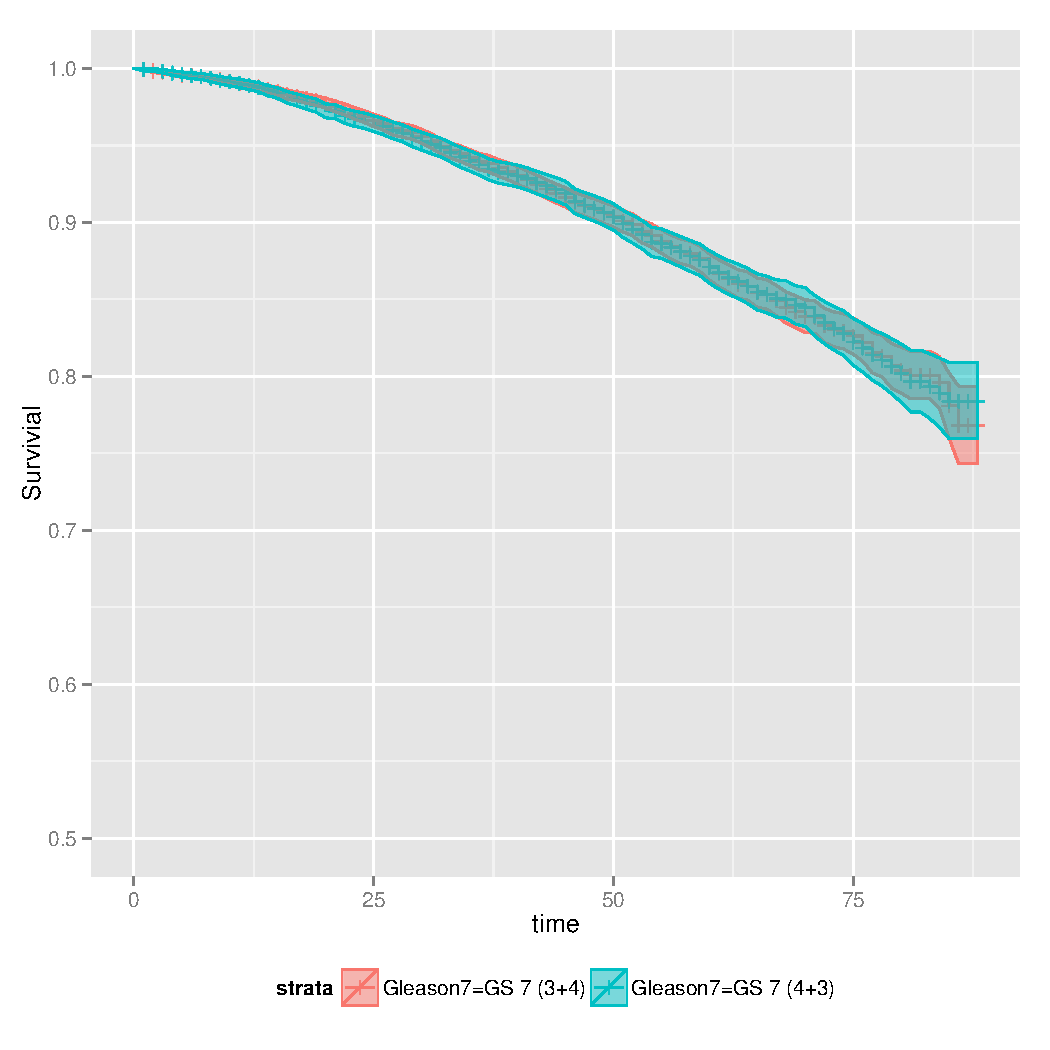
\includegraphics[width=\maxwidth]{figure/OS_Gleason7} 

}



\end{knitrout}

    \caption{(OS\_Gleason7.pdf) KM plot for OS by primary-secondary patterns
    within the 12,986 patients with a
    Gleason score of 7.}
    \label{fig:primary_secondary_km_7os}
  \end{subfigure}
  ~ 
  \begin{subfigure}[t]{0.48\textwidth}
\begin{knitrout}
\definecolor{shadecolor}{rgb}{0.969, 0.969, 0.969}\color{fgcolor}

{\centering 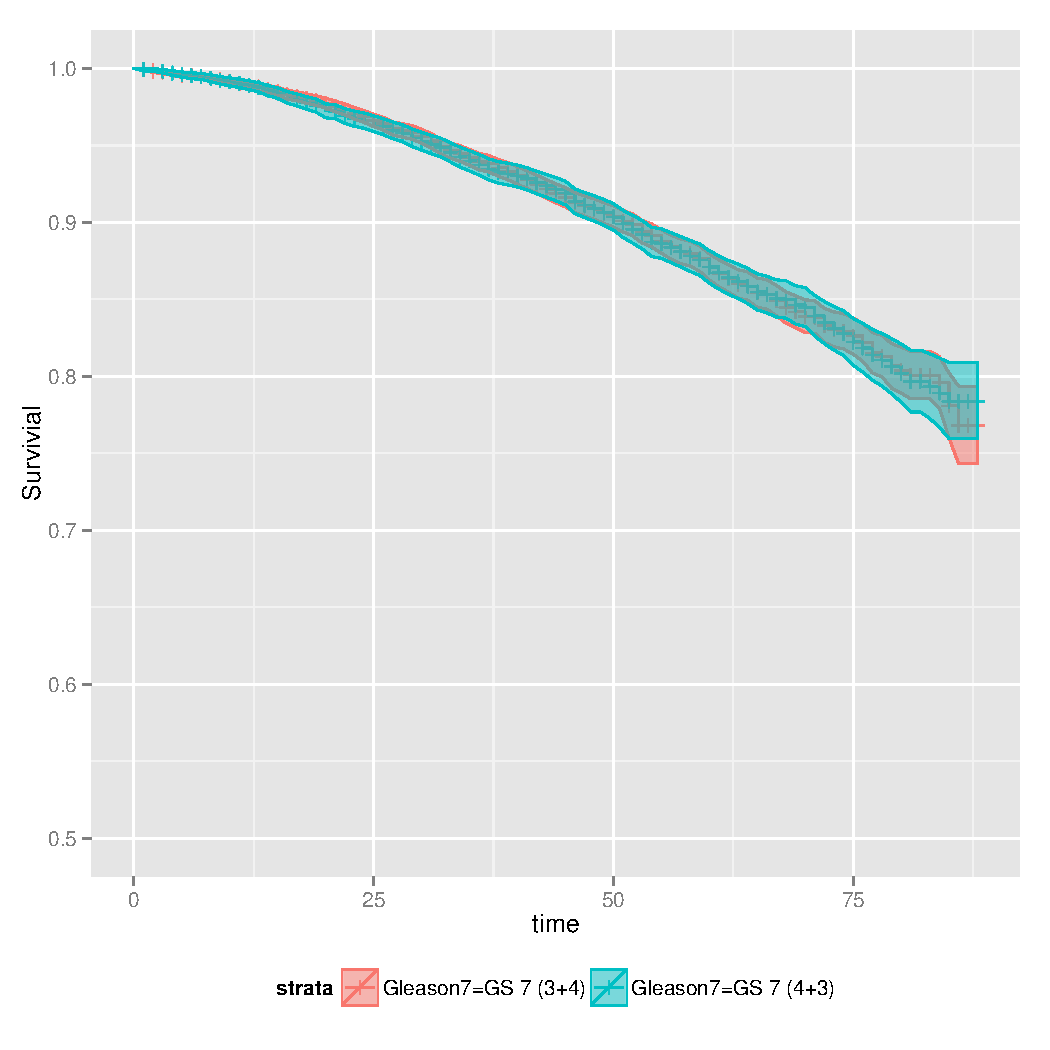
\includegraphics[width=\maxwidth]{figure/PCSS_Gleason7} 

}



\end{knitrout}

    \caption{(PCSS\_Gleason7.pdf) KM plot for PCSS by primary-secondary patterns
    within the
    12,986 patients with a Gleason score
    of 7.}
    \label{fig:primary_secondary_km_7pcss}
  \end{subfigure}
  \caption{KM plots for OS and PCSS by primary-secondary patterns for Gleason 7,
  See Table~\ref{tab:Gleason_primary_secondary_univar} for
  the log-rank test p-values.}
  \label{fig:primary_secondary_km}
\end{figure}
%}}}




%}}}

\subsubsection{Should the primary/secondary patterns be used in a multivariable
model?}  
%{{{










% in the appendix now
% % latex.default(temp, file = "../tex/os_pcss_coxph.tex", title = "",      ctable = TRUE, size = "tiny", caption = "Hazard ratios (HR) along with 95\\% confidence\n              intervals (LCL, UCL) and p-values for testing if the hazard ratio\n              is statistically different from 1 are presented in this table for\n              both univariable and multivariable regression models of both\n              overall survival and prostate cancer specific survival.",      label = "tab:os_pcss_coxph", cgroup = c("OS (univar)", "OS (multivar)",          "PCSS (univar)", "PCSS (multivar)"), n.crgoup = rep(4,          4), colhead = rep(c("HR", "LCL", "UCL", "p-value"), 4),      rgroup = rgrp, n.rgroup = nrgrp, rowname = rwnm, col.just = rep("r",          ncol(temp))) 
%
{\tiny\ctable[caption={Hazard ratios (HR) along with 95\% confidence
              intervals (LCL, UCL) and p-values for testing if the hazard ratio
              is statistically different from 1 are presented in this table for
              both univariable and multivariable regression models of both
              overall survival and prostate cancer specific survival.},label=tab:os_pcss_coxph,pos=!tbp,]{lrrrrcrrrrcrrrrcrrrr}{}{\FL
\multicolumn{1}{l}{\bfseries }&\multicolumn{4}{c}{\bfseries OS (univar)}&\multicolumn{1}{c}{\bfseries }&\multicolumn{4}{c}{\bfseries OS (multivar)}&\multicolumn{1}{c}{\bfseries }&\multicolumn{4}{c}{\bfseries PCSS (univar)}&\multicolumn{1}{c}{\bfseries }&\multicolumn{4}{c}{\bfseries PCSS (multivar)}\NN
\cline{2-5} \cline{7-10} \cline{12-15} \cline{17-20}
\multicolumn{1}{l}{}&\multicolumn{1}{c}{HR}&\multicolumn{1}{c}{LCL}&\multicolumn{1}{c}{UCL}&\multicolumn{1}{c}{p-value}&\multicolumn{1}{c}{}&\multicolumn{1}{c}{HR}&\multicolumn{1}{c}{LCL}&\multicolumn{1}{c}{UCL}&\multicolumn{1}{c}{p-value}&\multicolumn{1}{c}{}&\multicolumn{1}{c}{HR}&\multicolumn{1}{c}{LCL}&\multicolumn{1}{c}{UCL}&\multicolumn{1}{c}{p-value}&\multicolumn{1}{c}{}&\multicolumn{1}{c}{HR}&\multicolumn{1}{c}{LCL}&\multicolumn{1}{c}{UCL}&\multicolumn{1}{c}{p-value}\ML
{\bfseries Era}&&&&&&&&&&&&&&&&&&&\NN
~~Era 1&Reference&&&&&Reference&&&&&Reference&&&&&Reference&&&\NN
~~Era 2&0.83&0.76&0.90&\textless 0.001&&0.84&0.77&0.92&\textless 0.001&&0.83&0.76&0.90&\textless 0.001&&0.84&0.77&0.92&\textless 0.001\ML
{\bfseries Age}&&&&&&&&&&&&&&&&&&&\NN
~~[40,50)&Reference&&&&&Reference&&&&&Reference&&&&&Reference&&&\NN
~~[50,70)&0.95&0.84&1.09&0.481&&0.96&0.84&1.10&0.554&&0.95&0.84&1.09&0.481&&0.96&0.84&1.10&0.554\NN
~~[70,85]&1.62&1.44&1.81&\textless 0.001&&1.61&1.43&1.80&\textless 0.001&&1.62&1.44&1.81&\textless 0.001&&1.61&1.43&1.80&\textless 0.001\ML
{\bfseries T.Stage}&&&&&&&&&&&&&&&&&&&\NN
~~T Stage 1&Reference&&&&&Reference&&&&&Reference&&&&&Reference&&&\NN
~~T Stage 2&1.19&1.10&1.29&\textless 0.001&&1.12&1.03&1.21&0.006&&1.19&1.10&1.29&\textless 0.001&&1.12&1.03&1.21&0.006\NN
~~T Stage 3/4&1.54&1.34&1.77&\textless 0.001&&1.24&1.07&1.43&0.003&&1.54&1.34&1.77&\textless 0.001&&1.24&1.07&1.43&0.003\ML
{\bfseries PSA}&&&&&&&&&&&&&&&&&&&\NN
~~[0, 10) ng/ml&Reference&&&&&Reference&&&&&Reference&&&&&Reference&&&\NN
~~[10, 20) ng/ml&1.45&1.32&1.58&\textless 0.001&&1.36&1.24&1.49&\textless 0.001&&1.45&1.32&1.58&\textless 0.001&&1.36&1.24&1.49&\textless 0.001\NN
~~[20, Inf) ng/ml&1.62&1.47&1.78&\textless 0.001&&1.50&1.36&1.66&\textless 0.001&&1.62&1.47&1.78&\textless 0.001&&1.50&1.36&1.66&\textless 0.001\ML
{\bfseries Gleason7}&&&&&&&&&&&&&&&&&&&\NN
~~GS 7 (3+4)&Reference&&&&&Reference&&&&&Reference&&&&&Reference&&&\NN
~~GS 7 (4+3)&1.00&0.90&1.11&0.998&&0.99&0.90&1.10&0.915&&1.00&0.90&1.11&0.998&&0.99&0.90&1.10&0.915\NN
~~GS 8&1.34&1.21&1.48&\textless 0.001&&1.23&1.11&1.36&\textless 0.001&&1.34&1.21&1.48&\textless 0.001&&1.23&1.11&1.36&\textless 0.001\NN
~~GS 9&1.92&1.72&2.14&\textless 0.001&&1.72&1.54&1.92&\textless 0.001&&1.92&1.72&2.14&\textless 0.001&&1.72&1.54&1.92&\textless 0.001\NN
~~GS 10&2.74&2.16&3.47&\textless 0.001&&2.47&1.95&3.14&\textless 0.001&&2.74&2.16&3.47&\textless 0.001&&2.47&1.95&3.14&\textless 0.001\LL
}}


The results of the Cox proportional hazard regression models for overall
survival and prostate cancer specific survival are presented in
Table~\ref{tab:os_pcss_coxph} on page~\pageref{tab:os_pcss_coxph}.  Both
univariable and multivariable regression models are presented.  The univariable
models are built with only the noted predictor variable whereas the
multivariable models use the era, age, PSA, T Stage, and Gleason score jointly
as predictors for survival.




For overall survival we find that the patients diagnosed in Era 2
have better outcomes, i.e., longer survival, than those diagnosed
in the earlier Era 1.  For example, the hazard ratio between Era 2 and Era 1 for
overall survival based on the multivariable cox regression model is
0.84 (95\% CI: 0.77, 0.92; p \textless 0.001).

No statistically signficant difference in overall surverival was observed
between Gleason 7 (4+3) and Gleason 7 (3+4), HR = 0.99 (95\% CI: 0.90, 1.10; p = 0.915).  

Testing for a difference in the hazard ratio between sequential Gleason scores
is reported in Table~\ref{tab:sequential_hr}.  Considering that the data is
fictitious and the methods for deliniating 3+4 and 4+3 was a coin flip, it's not
surprsing that the hazard ratio between these two levels is not statistically
different from 1.  In general, and as expected for prostate cancer patients, as
the Gleason score increases the hazard increases as well.





%}}}





%=============%
% end of file %
%=============%

